\documentclass[11pt]{article}

\usepackage[margin=1in]{geometry}
\usepackage{amsmath}
\usepackage{amssymb}
\usepackage{booktabs}
\usepackage{hyperref}
\usepackage{listings}
\IfFileExists{microtype.sty}{\usepackage{microtype}}{}
\usepackage{xcolor}
\usepackage{tikz}
\usepackage{pgfplots}

\pgfplotsset{compat=1.18}

\hypersetup{
  colorlinks=true,
  linkcolor=blue,
  urlcolor=blue,
  citecolor=blue
}

\lstset{
  basicstyle=\ttfamily\small,
  breaklines=true,
  frame=single,
  columns=fullflexible
}

\newcommand{\axon}{Axon}
\newcommand{\rlm}{RLM}

\title{\axon: Do Recursive Scaffolds Help Short-Horizon Tasks Beyond Extra Iterations?}
\author{Anonymous Authors}
\date{}

\begin{document}
\maketitle

\begin{abstract}
Recursive Language Models are usually motivated by long-context and long-horizon reasoning \cite{zhang2025rlm,primeintellect2026rlm}. This paper asks a narrower operational question: \emph{for short-horizon tasks, does recursion help beyond simply giving non-recursive setups more attempts?}

We evaluate \axon, a Rust implementation of an \rlm-style scaffold, under controlled mode profiles and explicit evidence tiers. Axon extends recursion-only \rlm framing with checkpoint/restore, branch-style fork switching, and per-fork workspace state inside the sandbox loop. On a targeted short-horizon synthetic suite (8 tasks), depth1-iter3 and no-recursion-best-of-3 tie at 37.5\% pass while default and depth6-single-pass are 0\%, indicating that attempt budget matters more than depth alone. On a fixed non-synthetic Hugging Face smoke slice (40 runs), typed deterministic scoring raises measured pass rate from 10.0\% to 75.0\%, and runtime hardening reduces hard errors from 7 to 1 while leaving a single timeout. On the runtime-hardened slice, depth1-iter3 has the strongest mean dataset pass rate (100\%), no-recursion-best-of-3 is close (90\%), default is lower (60\%), and depth6-single-pass underperforms (50\%).

For Codeforces-like strict executable tasks (8 matched runs), a strict Rust-only output contract yields 4/8 strict passes and zero hard runtime errors; remaining failures are compile rejects. Long-context suites are used as stress context rather than the main claim target: books depth-profile measurements favor iteration-rich profiles, while ledger evidence remains mixed and partially incomplete for full four-profile comparison. Overall, current evidence supports a calibrated claim: shallow recursion can help, but gains are tightly coupled to attempt budget, evaluator design, and output-contract compliance.
\end{abstract}

\section{Introduction}
Long-context degradation remains a recurring challenge even for models with large nominal windows \cite{hong2025contextrot}. Recent agent-style work therefore externalizes reasoning into tool loops \cite{yao2023react,wang2024codeact} and studies longer-horizon software tasks \cite{jimenez2024swebench,metr2025rebench}. Within this direction, \rlm emphasizes recursive decomposition and context folding \cite{zhang2025rlm}, with follow-up engineering reports arguing that recursive delegation can preserve main-trajectory focus \cite{primeintellect2026rlm}. Recent scaling studies further argue that architecture-task alignment and coordination overhead, not agent count alone, determine multi-agent gains \cite{kim2025scaling,google2026agentscaling}. Related analyses of long chain-of-thought trajectories also suggest that stable sub-structure, not only raw depth, may drive reliability \cite{chen2026molecular}.

Most prior framing, however, centers on long-horizon settings. In practical deployment, many workloads are short-horizon but strict: they demand exact formatting, deterministic checking, and low failure rates. This motivates our main question:

\begin{quote}
\textbf{RQ:} When horizon is short, does recursion provide measurable benefit beyond giving a non-recursive setup more iterations?
\end{quote}

We study this question using \axon, an open Rust implementation of an \rlm-style scaffold with sandboxed execution and deterministic benchmark harnessing (implementation details and code: \url{https://github.com/diogenesoftoronto/axon}).

\paragraph{Main findings.}
\begin{enumerate}
  \item \textbf{Depth alone is weak:} deep single-pass recursion (depth6-single-pass) is consistently poor on short-horizon slices.
  \item \textbf{Attempt budget is first-order:} depth1-iter3 and no-recursion-best-of-3 usually dominate single-pass variants.
  \item \textbf{Measurement policy is first-order:} typed lenient checks change HF measured pass from 10\% to 75\% on the same 40 runs.
  \item \textbf{Runtime hardening helps but does not remove all systems risk:} hard errors drop from 7 to 1, with one residual timeout.
  \item \textbf{Executable bottleneck shifted:} Codeforces-like failures moved from runtime crashes to compile-quality and output-contract compliance.
\end{enumerate}

\section{System and Comparison Setup}
\axon implements a recursive controller that can call a child model loop and run sandboxed Python tools between reasoning steps. For this paper, we treat implementation as fixed and vary only mode profiles.

\begin{table}[h]
\centering
\caption{Mode profiles used for recursion-vs-iterations comparisons.}
\label{tab:modes}
\begin{tabular}{lccp{6.4cm}}
\toprule
Mode & Max depth & Max iterations & Interpretation \\
\midrule
current-default & 0 & 1 & non-recursive single-pass baseline \\
current-no-recursion-best-of-3 & 0 & 3 & more attempts without recursion \\
current-depth6-single-pass & 6 & 1 & deep recursion with minimal attempt budget \\
current-depth1-iter3 & 1 & 3 & shallow recursion plus larger attempt budget \\
\bottomrule
\end{tabular}
\end{table}

This table defines the core experimental axis: recursion depth versus attempt budget.

Depth-profile comparisons are prompt-neutral in the benchmark harness: for non-Codeforces tasks, all modes receive the same task query and context text, and mode differences are introduced only via runtime controls (max depth and max iterations). The only mode-independent query augmentation is the strict Rust-output contract used for \texttt{rust\_exec\_exact} tasks.

\subsection{Checkpointed Branching State as an Axon Extension}
Relative to recursion-centric \rlm descriptions \cite{zhang2025rlm,primeintellect2026rlm}, Axon exposes explicit state-management operators inside each sandbox loop: \texttt{CHECKPOINT\_CREATE}/\texttt{CHECKPOINT\_RESTORE} for recoverable snapshots, \texttt{FORK\_CREATE}/\texttt{FORK\_SWITCH}/\texttt{FORK\_LIST} for branch navigation, \texttt{VFS\_WRITE}/\texttt{VFS\_READ}/\texttt{VFS\_LIST} for per-branch scratch state, and \texttt{STRATEGY\_COMMIT}/\texttt{STRATEGY\_STATUS} for rationale tracking.

This shifts the agent from pure recursive delegation toward checkpointed exploratory search with reversible branch-local state. In this paper, these controls are held fixed across all profiles; mode comparisons therefore isolate depth/iteration settings rather than a checkpointing ablation.

\section{Benchmarks and Evidence Policy}
\subsection{Benchmark Families}
We use four benchmark families, each serving a distinct role.

\textbf{Short-horizon mode discrimination (synthetic, 8 tasks).} Small deterministic tasks designed to separate profile behavior under strict matching.

\textbf{Short-horizon external benchmarks (non-synthetic HF slice, 40 runs).} Five Hugging Face-derived packs, two tasks per pack, four modes. These runs are used for evaluator and runtime ablations under fixed workload.

\textbf{Strict executable coding (Codeforces-like, 8 runs).} Two tasks across four modes with compile-and-run validation.

\textbf{Long-context stress suites (books, ledger).} Used as context and stress tests, not as sole basis for short-horizon claims.

\subsection{Books and Ledger Intent}
Books+distractors evaluates retrieval under semantic interference: overlapping entities and narratives force selective grounding rather than keyword lookup. Ledger evaluates exact dense aggregation over large record sets, emphasizing coverage, arithmetic correctness, and output contract adherence. Together, they probe different failure modes in long contexts.

\subsection{Hugging Face Pack Characteristics}
\begin{table}[h]
\centering
\caption{Hugging Face-derived benchmark packs currently integrated.}
\label{tab:hf-packs}
\begin{tabular}{lrrr}
\toprule
Dataset pack & Tasks & Avg context chars & Avg query chars \\
\midrule
GSM8K subset & 100 & 64.0 & 231.3 \\
MBPP calls subset & 100 & 59.0 & 311.4 \\
ARC-Challenge subset & 100 & 52.0 & 398.2 \\
BoolQ subset & 100 & 554.9 & 77.0 \\
HellaSwag subset & 100 & 38.0 & 475.3 \\
\bottomrule
\end{tabular}
\end{table}

\subsection{Evidence Tiering}
We separate claims by evidence strength:
\begin{itemize}
  \item \textbf{Tier A (higher confidence):} repeated long-context suites and controlled intervention contrasts.
  \item \textbf{Tier B (diagnostic):} small smoke slices (HF 40 runs total, Codeforces 8 runs total).
\end{itemize}
Tier B is used for mechanism discovery and hypothesis refinement, not broad capability claims.

\section{Results: Short-Horizon Recursion vs Iterations}
\subsection{Head-to-Head Profile Outcomes}
Table \ref{tab:sh-core} summarizes the three short-horizon slices most relevant to the research question.

\begin{table}[t]
\centering
\caption{Short-horizon mode comparison across three slices.}
\label{tab:sh-core}
\begin{tabular}{lccc}
\toprule
Mode & Targeted synthetic (8 tasks) & HF hardened-runtime mean (5 packs) & Codeforces strict (2 tasks) \\
\midrule
current-default & 0.0\% & 60.0\% & 50.0\% \\
current-depth1-iter3 & 37.5\% & 100.0\% & 100.0\% \\
current-depth6-single-pass & 0.0\% & 50.0\% & 0.0\% \\
current-no-recursion-best-of-3 & 37.5\% & 90.0\% & 50.0\% \\
\bottomrule
\end{tabular}
\end{table}

\begin{figure}[t]
\centering
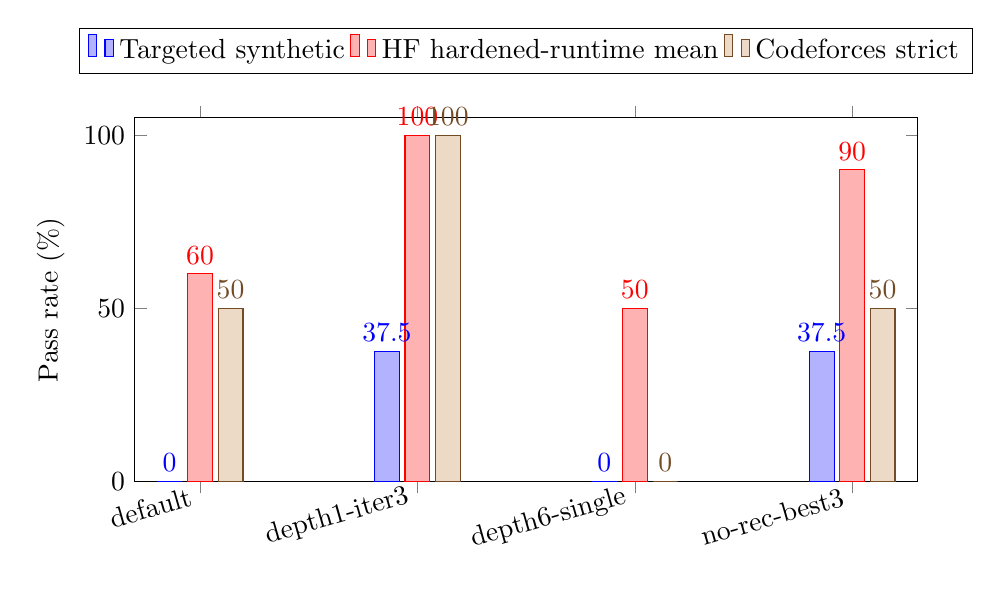
\begin{tikzpicture}
\begin{axis}[
  ybar,
  bar width=9pt,
  width=0.95\linewidth,
  height=6.2cm,
  ymin=0,
  ymax=105,
  ylabel={Pass rate (\%)},
  symbolic x coords={default,depth1-iter3,depth6-single,no-rec-best3},
  xtick=data,
  x tick label style={rotate=16,anchor=east},
  legend style={at={(0.5,1.12)},anchor=south,legend columns=3},
  nodes near coords,
  nodes near coords align={vertical}
]
\addplot coordinates {(default,0) (depth1-iter3,37.5) (depth6-single,0) (no-rec-best3,37.5)};
\addplot coordinates {(default,60) (depth1-iter3,100) (depth6-single,50) (no-rec-best3,90)};
\addplot coordinates {(default,50) (depth1-iter3,100) (depth6-single,0) (no-rec-best3,50)};
\legend{Targeted synthetic,HF hardened-runtime mean,Codeforces strict}
\end{axis}
\end{tikzpicture}
\caption{Short-horizon mode comparison across three evaluation slices.}
\label{fig:short-horizon-modes}
\end{figure}

Two patterns are consistent. First, deep single-pass recursion underperforms despite higher depth. Second, increasing attempt budget is the dominant gain source; both iteration-rich profiles outperform single-pass profiles on most slices. Shallow recursion with attempts (depth1-iter3) is strongest in these measurements, but non-recursive best-of-3 is often close.

\subsection{Analytical Framing: Attempts, Coordination, and Structure}
To connect our measurements to agent-scaling theory, we use a compact decomposition inspired by the alignment and tool-coordination principles in \cite{kim2025scaling,google2026agentscaling}.

Let \(p_1\) denote single-attempt success for a fixed mode family. Under an independence approximation, a \(k\)-attempt non-recursive baseline is
\[
A_k(p_1) = 1 - (1-p_1)^k.
\]
Observed pass can then be written as
\[
\hat p = s_{\text{check}}\,(1-e_{\text{runtime}})\,p_{\text{task}},
\]
where \(s_{\text{check}}\) captures checker sensitivity (strict vs typed), \(e_{\text{runtime}}\) is runtime failure probability, and \(p_{\text{task}}\) is latent task-solving probability.

For equal attempt budget \((k=3)\), we define recursion lift as
\[
L_{\text{rec}} = p(d{=}1,k{=}3) - p(d{=}0,k{=}3).
\]
We interpret \(L_{\text{rec}}\) using
\[
p_{\text{task}} \approx A_k(p_1) + \lambda\,\mathcal{M} - \tau,
\]
where \(\mathcal{M}\) is a reasoning-structure term (stable deep-reasoning, reflection, and exploration motifs, consistent with \cite{chen2026molecular}) and \(\tau\) is coordination tax (sequential dependence and tool overhead) \cite{kim2025scaling}.

\begin{table}[t]
\centering
\caption{Attempt-only baseline check using \(A_3(p_1)=1-(1-p_1)^3\) against observed no-recursion-best-of-3 pass.}
\label{tab:attempt-baseline}
\begin{tabular}{lrrr}
\toprule
Slice & \(p_1\) from default & \(A_3(p_1)\) predicted & Observed no-rec best-of-3 \\
\midrule
Targeted synthetic & 0.000 & 0.000 & 0.375 \\
HF hardened mean & 0.600 & 0.936 & 0.900 \\
Books depth-profile & 0.200 & 0.488 & 0.800 \\
Codeforces strict & 0.500 & 0.875 & 0.500 \\
\bottomrule
\end{tabular}
\end{table}

The table shows the independence baseline is only partially descriptive: it is close on HF, optimistic on Codeforces, and pessimistic on books. This pattern is consistent with a task-dependent coordination term \(\tau\) and non-independent retries.

\begin{figure}[t]
\centering
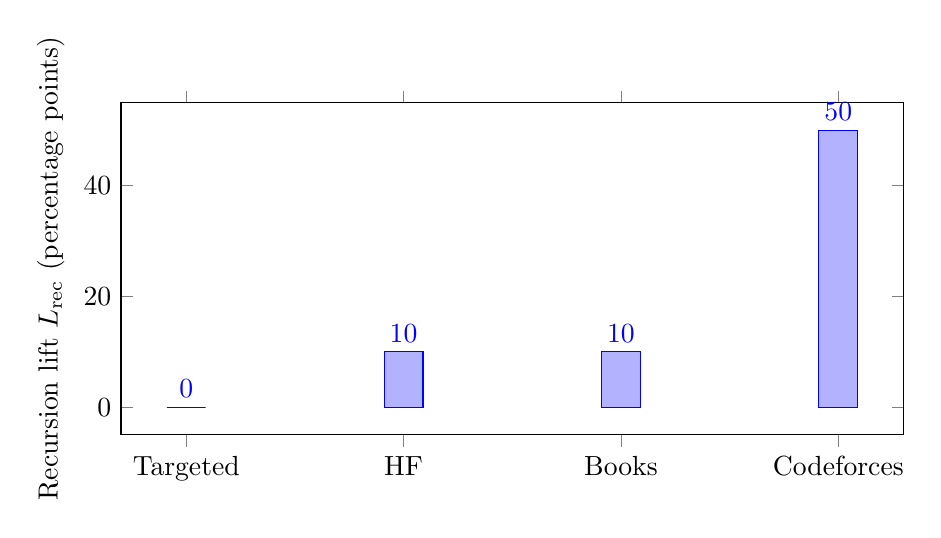
\begin{tikzpicture}
\begin{axis}[
  ybar,
  bar width=14pt,
  width=0.95\linewidth,
  height=5.8cm,
  ymin=-5,
  ymax=55,
  ylabel={Recursion lift \(L_{\text{rec}}\) (percentage points)},
  symbolic x coords={Targeted,HF,Books,Codeforces},
  xtick=data,
  nodes near coords,
  nodes near coords align={vertical}
]
\addplot coordinates {(Targeted,0) (HF,10) (Books,10) (Codeforces,50)};
\end{axis}
\end{tikzpicture}
\caption{Equal-budget recursion lift \(L_{\text{rec}}\): depth1-iter3 minus no-recursion-best-of-3.}
\label{fig:recursion-lift}
\end{figure}

Figure \ref{fig:short-horizon-modes} and Figure \ref{fig:recursion-lift} align with the Google scaling view: deeper coordination without sufficient budget can underperform, while aligned shallow coordination can help \cite{kim2025scaling,google2026agentscaling}. Figure \ref{fig:hf-policy-stack} maps primarily to \(s_{\text{check}}\) and \(e_{\text{runtime}}\), showing that measured reliability depends strongly on evaluation/runtime policy in addition to latent task-solving quality.
Interpreting \(\mathcal{M}\) through \cite{chen2026molecular}, Figure \ref{fig:recursion-lift} can be read as an empirical proxy for when recursive calls preserve useful long-reasoning structure versus when coordination overhead dominates.

\subsection{Scoring Policy and Runtime Robustness as Separate Effects}
To avoid mixing quality changes with measurement changes, we evaluate strict scoring, typed-lenient scoring, and runtime hardening on the exact same HF workload (40 runs).

\begin{table}[t]
\centering
\caption{HF fixed-slice outcomes under scoring/runtime variants (40 runs).}
\label{tab:hf-robustness}
\begin{tabular}{lrrrr}
\toprule
Configuration & Passes & Mismatches & Errors & Pass rate \\
\midrule
Strict checker + runtime policy A & 4 & 29 & 7 & 10.0\% \\
Typed checker + runtime policy A & 30 & 8 & 2 & 75.0\% \\
Typed checker + runtime policy B (hardened) & 30 & 9 & 1 & 75.0\% \\
\bottomrule
\end{tabular}
\end{table}

\begin{figure}[t]
\centering
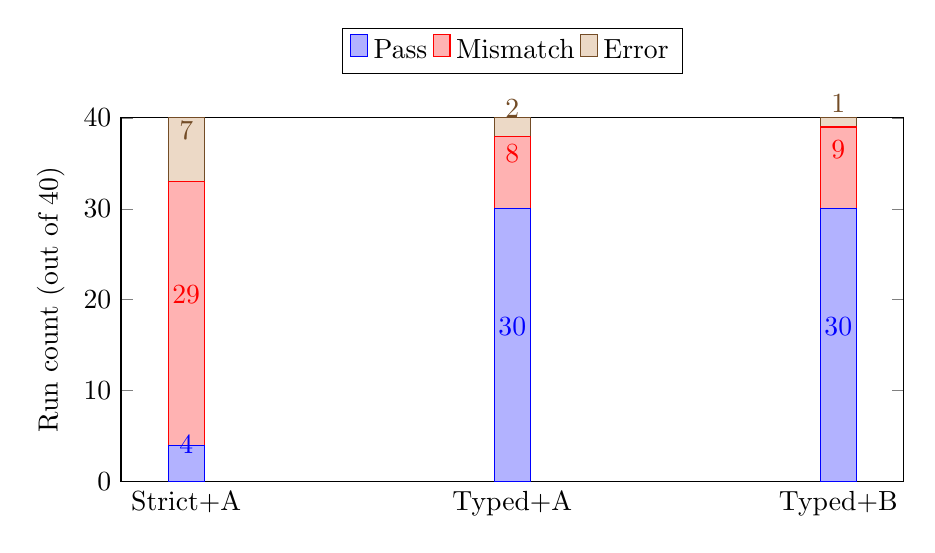
\begin{tikzpicture}
\begin{axis}[
  ybar stacked,
  bar width=13pt,
  width=0.95\linewidth,
  height=6.2cm,
  ymin=0,
  ymax=40,
  ylabel={Run count (out of 40)},
  symbolic x coords={StrictA,TypedA,TypedB},
  xtick=data,
  xticklabels={Strict+A,Typed+A,Typed+B},
  legend style={at={(0.5,1.12)},anchor=south,legend columns=3},
  nodes near coords,
  nodes near coords align={vertical}
]
\addplot coordinates {(StrictA,4) (TypedA,30) (TypedB,30)};
\addplot coordinates {(StrictA,29) (TypedA,8) (TypedB,9)};
\addplot coordinates {(StrictA,7) (TypedA,2) (TypedB,1)};
\legend{Pass,Mismatch,Error}
\end{axis}
\end{tikzpicture}
\caption{HF fixed-slice outcomes under scoring and runtime policies.}
\label{fig:hf-policy-stack}
\end{figure}

Interpretation is direct: typed checks (including near-miss matching where appropriate) are the main reason measured reliability increases on this slice. Runtime hardening primarily reduces hard failures, from 7 to 1, while preserving pass count. The remaining hard failure is a timeout, so timeout behavior remains an explicit residual systems issue.

\subsection{HF Mode Matrix on Runtime-Hardened Slice}
\begin{table}[t]
\centering
\caption{Runtime-hardened HF pass rates (\%) by dataset and mode.}
\label{tab:hf-matrix}
\begin{tabular}{lrrrr}
\toprule
Dataset & default & depth1-iter3 & depth6-single-pass & no-recursion-best-of-3 \\
\midrule
ARC-Challenge & 50 & 100 & 50 & 100 \\
BoolQ & 100 & 100 & 50 & 100 \\
GSM8K & 0 & 100 & 0 & 100 \\
HellaSwag & 100 & 100 & 50 & 50 \\
MBPP calls & 50 & 100 & 100 & 100 \\
\midrule
Mean across datasets & 60 & 100 & 50 & 90 \\
\bottomrule
\end{tabular}
\end{table}

Because each cell is based on two tasks, this matrix is directional rather than definitive. Still, it matches the broader short-horizon pattern: depth without attempts is weak, and attempt-rich profiles are stronger.

\subsection{Codeforces-Like Strict Executable Tasks}
Two prompt-contract conditions were evaluated on matched 8-run Codeforces-like slices: a standard contract and a strict Rust-only contract with explicit invalid non-Rust examples.

\begin{table}[t]
\centering
\caption{Codeforces-like strict executable outcomes under two prompt-contract conditions.}
\label{tab:cf-contract-comparison}
\begin{tabular}{lrr}
\toprule
Metric & Standard contract & Strict Rust-only contract \\
\midrule
Strict compile-and-run passes & 0/8 (0.0\%) & 4/8 (50.0\%) \\
Hard engine errors & 4/8 (50.0\%) & 0/8 (0.0\%) \\
Completed but unmatched & 4/8 (50.0\%) & 4/8 (50.0\%) \\
\bottomrule
\end{tabular}
\end{table}

\begin{figure}[t]
\centering
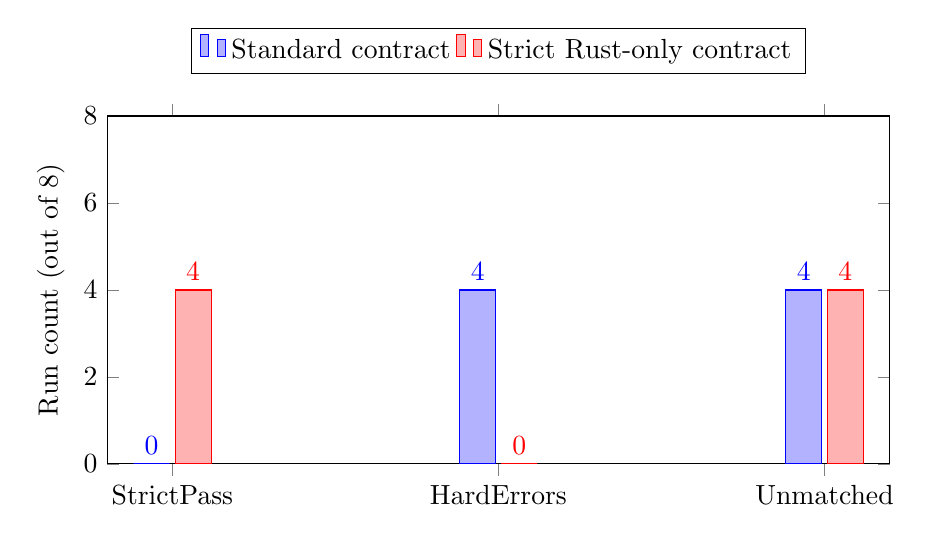
\begin{tikzpicture}
\begin{axis}[
  ybar,
  bar width=13pt,
  width=0.95\linewidth,
  height=6cm,
  ymin=0,
  ymax=8,
  ylabel={Run count (out of 8)},
  symbolic x coords={StrictPass,HardErrors,Unmatched},
  xtick=data,
  legend style={at={(0.5,1.12)},anchor=south,legend columns=2},
  nodes near coords,
  nodes near coords align={vertical}
]
\addplot coordinates {(StrictPass,0) (HardErrors,4) (Unmatched,4)};
\addplot coordinates {(StrictPass,4) (HardErrors,0) (Unmatched,4)};
\legend{Standard contract,Strict Rust-only contract}
\end{axis}
\end{tikzpicture}
\caption{Codeforces-like outcome shift under prompt-contract conditions.}
\label{fig:cf-contract-shift}
\end{figure}

Under the strict contract condition, remaining misses are compile rejects rather than runtime crashes.

\begin{table}[t]
\centering
\caption{Compile-reject taxonomy under the strict Rust-only contract condition (4 rejects).}
\label{tab:cf-taxonomy}
\begin{tabular}{lrr}
\toprule
Reject class & Count & Share \\
\midrule
Non-Rust or generic fenced REPL/Python-style output & 3 & 75\% \\
Rust type mismatch (bitmask \texttt{usize} vs \texttt{u32}) & 1 & 25\% \\
\bottomrule
\end{tabular}
\end{table}

For the short-horizon question, this supports a practical conclusion: recursive scaffolds help only if the final artifact channel remains contract-compliant.

\section{Long-Context Results as Stress Context}
\subsection{Books Depth-Profile Measurement}
A dedicated books depth-profile measurement (10 tasks per mode) is aligned with the short-horizon mode set.

\begin{table}[t]
\centering
\caption{Books+distractors depth/iteration profile results (10 tasks per mode).}
\label{tab:books-depth}
\begin{tabular}{lcc}
\toprule
Mode & Pass rate & 95\% CI \\
\midrule
current-default & 20.0\% & [5.67, 50.98] \\
current-depth1-iter3 & 90.0\% & [59.58, 98.21] \\
current-depth6-single-pass & 20.0\% & [5.67, 50.98] \\
current-no-recursion-best-of-3 & 80.0\% & [49.02, 94.33] \\
\bottomrule
\end{tabular}
\end{table}

\begin{figure}[t]
\centering
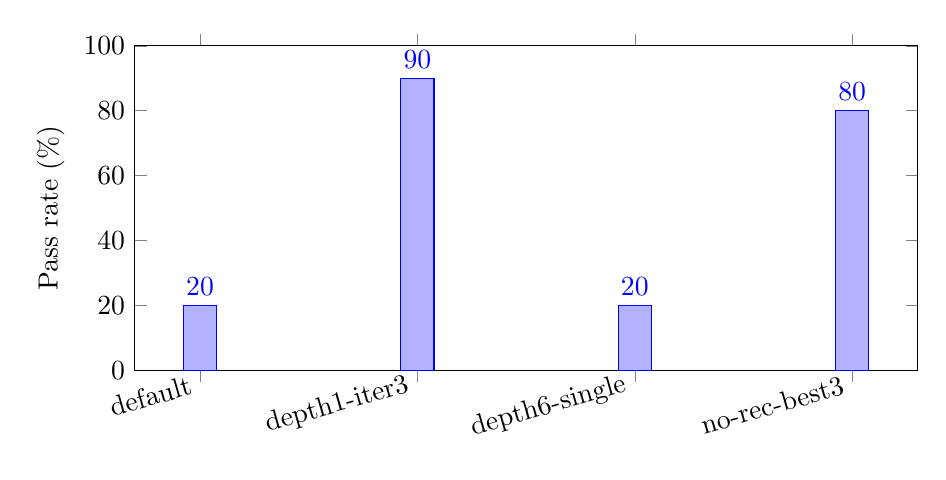
\begin{tikzpicture}
\begin{axis}[
  ybar,
  bar width=12pt,
  width=0.95\linewidth,
  height=5.7cm,
  ymin=0,
  ymax=100,
  ylabel={Pass rate (\%)},
  symbolic x coords={default,depth1-iter3,depth6-single,no-rec-best3},
  xtick=data,
  x tick label style={rotate=16,anchor=east},
  nodes near coords,
  nodes near coords align={vertical}
]
\addplot coordinates {(default,20) (depth1-iter3,90) (depth6-single,20) (no-rec-best3,80)};
\end{axis}
\end{tikzpicture}
\caption{Books+distractors depth-profile pass rates (10 tasks per mode).}
\label{fig:books-depth-bars}
\end{figure}

This long-context measurement is consistent with the short-horizon pattern: iteration-rich profiles dominate single-pass profiles; shallow recursion plus attempts is best on this slice, with substantial overlap in uncertainty intervals.

\subsection{Ledger Status and Interpretation Limits}
Ledger evidence is currently split across two non-identical measurement sets. One set reports default 61.11\%, low-budget 44.44\%, and no-recursion 83.33\%. A second set reports depth1-iter3 at 57.14\% over 7 runs. Because profile coverage and run composition differ across these sets, this does not yet provide a consolidated four-profile ledger ranking.

Therefore, ledger supports heterogeneity and failure analysis, but not a final profile ranking under the new recursion-vs-iterations framing.

\section{Multi-Model Pareto Analysis Across Synthetic Providers}

To test whether our findings generalize beyond the default MiniMax-M2.5 model, we ran the targeted mode-profile benchmark (8 tasks, 4 modes) across seven models available on the Synthetic inference platform: MiniMax-M2.1, MiniMax-M2.5, Qwen3.5-397B-A17B, Qwen3-235B-A22B-Thinking-2507, DeepSeek-V3.2, Kimi-K2-Thinking, and Kimi-K2.5. All models use OpenAI-compatible endpoints at uniform \$0.0000003--\$0.000003/token pricing, enabling direct cost comparison.

\paragraph{FINAL extraction fix.} During multi-model evaluation, we discovered a bug in the RLM engine fallback path: when all iterations exhausted without the model producing a \texttt{FINAL()} directive during the loop body, the engine issued a final prompt and returned the raw LLM text without extracting \texttt{FINAL()} content. This caused correct answers like \texttt{FINAL(88492)} to fail exact matching. After fixing this, depth6-single-pass results improved substantially for models that reliably emit \texttt{FINAL()} markers (particularly Kimi-K2.5, from 0\% to 62.5\%). The six-model results below were collected \emph{before} this fix; the Kimi-K2.5 results include the fix.

\subsection{Cross-Model Mode Comparison}

\begin{table}[t]
\centering
\caption{Pass rate (\%) by model and mode on the targeted 8-task profile suite (224 total runs).}
\label{tab:multimodel-passrate}
\begin{tabular}{lrrrr}
\toprule
Model & default & depth1-iter3 & depth6-single & no-rec-best3 \\
\midrule
MiniMax-M2.1 & 0.0 & 37.5 & 0.0 & 37.5 \\
MiniMax-M2.5 & 0.0 & 37.5 & 0.0 & 50.0 \\
Qwen3.5-397B & 0.0 & \textbf{75.0} & 0.0 & 12.5 \\
Qwen3-235B-Think & 0.0 & 37.5 & 0.0 & 25.0 \\
DeepSeek-V3.2 & 0.0 & 50.0 & 0.0 & 37.5 \\
Kimi-K2-Think & 0.0 & 37.5 & 0.0 & 25.0 \\
\midrule
\multicolumn{5}{l}{\emph{Post-FINAL-fix:}} \\
Kimi-K2.5 & \textbf{62.5} & 50.0 & \textbf{62.5} & \textbf{75.0} \\
\bottomrule
\end{tabular}
\end{table}

\begin{figure}[t]
\centering
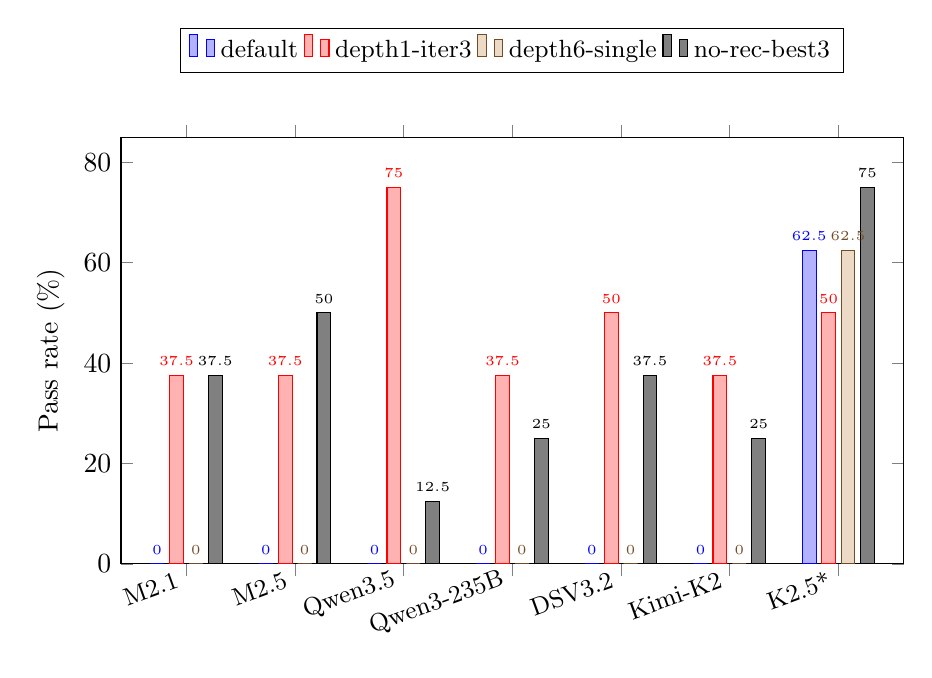
\begin{tikzpicture}
\begin{axis}[
  ybar,
  bar width=5pt,
  width=0.95\linewidth,
  height=7cm,
  ymin=0,
  ymax=85,
  ylabel={Pass rate (\%)},
  symbolic x coords={M2.1,M2.5,Qwen3.5,Qwen3-235B,DSV3.2,Kimi-K2,K2.5*},
  xtick=data,
  x tick label style={rotate=20,anchor=east,font=\small},
  legend style={at={(0.5,1.15)},anchor=south,legend columns=4,font=\small},
  nodes near coords,
  nodes near coords align={vertical},
  every node near coord/.append style={font=\tiny}
]
\addplot coordinates {(M2.1,0) (M2.5,0) (Qwen3.5,0) (Qwen3-235B,0) (DSV3.2,0) (Kimi-K2,0) (K2.5*,62.5)};
\addplot coordinates {(M2.1,37.5) (M2.5,37.5) (Qwen3.5,75) (Qwen3-235B,37.5) (DSV3.2,50) (Kimi-K2,37.5) (K2.5*,50)};
\addplot coordinates {(M2.1,0) (M2.5,0) (Qwen3.5,0) (Qwen3-235B,0) (DSV3.2,0) (Kimi-K2,0) (K2.5*,62.5)};
\addplot coordinates {(M2.1,37.5) (M2.5,50) (Qwen3.5,12.5) (Qwen3-235B,25) (DSV3.2,37.5) (Kimi-K2,25) (K2.5*,75)};
\legend{default,depth1-iter3,depth6-single,no-rec-best3}
\end{axis}
\end{tikzpicture}
\caption{Cross-model pass rates on the targeted 8-task suite. For the first six models (pre-fix), default and depth6-single-pass always score 0\%. Kimi-K2.5 (*post-FINAL-fix) breaks this pattern with 62.5\% in both default and depth6-single-pass.}
\label{fig:multimodel-passrate}
\end{figure}

Two structural findings hold across the six pre-fix models. First, \textbf{default (depth0, iter1) and depth6-single-pass both score 0\% universally}---no model can solve these tasks in a single unscaffolded pass, confirming that the task suite discriminates between modes, not just model quality. Second, \textbf{attempt-rich modes always outperform single-pass}. The specific ranking between depth1-iter3 and no-recursion-best-of-3 is model-dependent: Qwen3.5-397B strongly favors shallow recursion (75\% vs 12.5\%), while MiniMax-M2.5 favors pure iteration (50\% vs 37.5\%).

\textbf{Kimi-K2.5 (post-fix)} breaks both patterns: it scores 62.5\% in default mode and 62.5\% in depth6-single-pass, demonstrating that a sufficiently capable model can solve these tasks even in a single pass---\emph{provided the scaffold correctly extracts its answers}. Its best mode is no-recursion-best-of-3 at 75\%, matching the overall leader. Notably, K2.5 achieves all four readiness classifications as ``Promising'' (composite $>70$), the only model to do so across all modes.

\subsection{Speed and Cost Analysis}

\begin{table}[t]
\centering
\caption{Latency and cost per task in depth1-iter3 mode (best overall mode).}
\label{tab:multimodel-speed}
\begin{tabular}{lrrrr}
\toprule
Model & Avg time (s) & Avg tokens & Avg cost (USD) & OK rate (\%) \\
\midrule
MiniMax-M2.1 & \textbf{7.4} & 5786 & \textbf{0.0026} & 100 \\
MiniMax-M2.5 & 17.2 & 5257 & 0.0063 & 100 \\
Qwen3.5-397B & 11.9 & \textbf{4862} & 0.0044 & 100 \\
Qwen3-235B-Think & 36.4 & 5427 & 0.0095 & 100 \\
DeepSeek-V3.2 & 50.8 & 9995 & 0.0093 & 87.5 \\
Kimi-K2-Think & 71.7 & 8318 & 0.0093 & 75.0 \\
\midrule
\multicolumn{5}{l}{\emph{Post-FINAL-fix (best mode = no-rec-best3):}} \\
Kimi-K2.5 & 38.1 & 5487 & 0.0064 & 100 \\
\bottomrule
\end{tabular}
\end{table}

Speed varies by 10$\times$ across models: MiniMax-M2.1 averages 7.4s per task while Kimi-K2-Thinking averages 71.7s. Qwen3.5-397B achieves the best combination of speed (11.9s), quality (75\% pass), and cost (\$0.0044/task). Kimi-K2.5 (post-fix) matches the 75\% pass rate at moderate latency (38.1s) and cost (\$0.0064/task) with perfect 100\% reliability.

\subsection{Pareto Frontier: Quality vs Cost}

\begin{figure}[t]
\centering
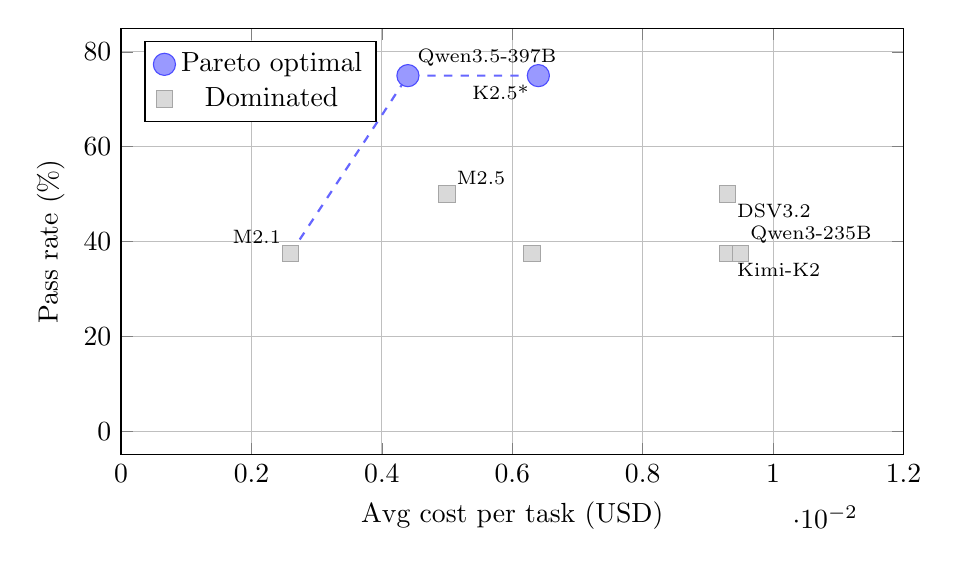
\begin{tikzpicture}
\begin{axis}[
  width=0.95\linewidth,
  height=7cm,
  xlabel={Avg cost per task (USD)},
  ylabel={Pass rate (\%)},
  xmin=0,
  xmax=0.012,
  ymin=-5,
  ymax=85,
  grid=major,
  scatter/classes={
    pareto={mark=*,draw=blue!70,fill=blue!40,mark size=4pt},
    dominated={mark=square*,draw=gray!70,fill=gray!30,mark size=3pt}
  },
  legend style={at={(0.03,0.97)},anchor=north west}
]
\addplot[scatter,only marks,scatter src=explicit symbolic] coordinates {
  (0.0026,37.5) [dominated]
  (0.0044,75.0) [pareto]
  (0.005,50.0) [dominated]
  (0.0063,37.5) [dominated]
  (0.0064,75.0) [pareto]
  (0.0093,50.0) [dominated]
  (0.0093,37.5) [dominated]
  (0.0095,37.5) [dominated]
};
\node[anchor=south west,font=\scriptsize] at (axis cs:0.0044,75) {Qwen3.5-397B};
\node[anchor=south east,font=\scriptsize] at (axis cs:0.0026,37.5) {M2.1};
\node[anchor=south west,font=\scriptsize] at (axis cs:0.005,50) {M2.5};
\node[anchor=north west,font=\scriptsize] at (axis cs:0.0093,50) {DSV3.2};
\node[anchor=north west,font=\scriptsize] at (axis cs:0.0093,37.5) {Kimi-K2};
\node[anchor=south west,font=\scriptsize] at (axis cs:0.0095,37.5) {Qwen3-235B};
\node[anchor=north east,font=\scriptsize] at (axis cs:0.0064,75) {K2.5*};
\draw[dashed,blue!60,thick] (axis cs:0.0026,37.5) -- (axis cs:0.0044,75.0) -- (axis cs:0.0064,75.0);
\legend{Pareto optimal,Dominated}
\end{axis}
\end{tikzpicture}
\caption{Pareto frontier of pass rate vs cost per task (best mode per model). Qwen3.5-397B and Kimi-K2.5 (*post-fix) tie at 75\% pass; Qwen3.5 is cheaper. MiniMax-M2.1 is the budget alternative.}
\label{fig:pareto-cost}
\end{figure}

\begin{figure}[t]
\centering
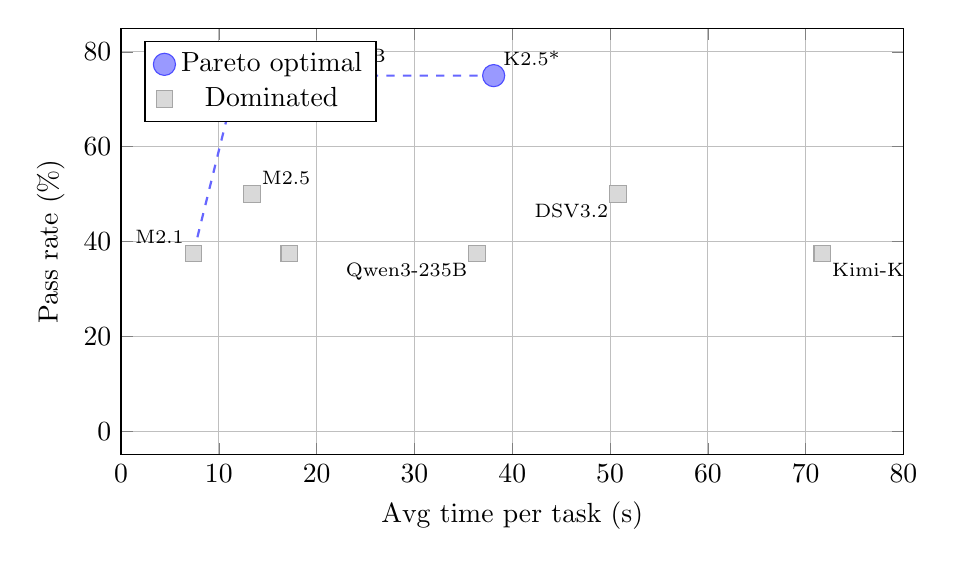
\begin{tikzpicture}
\begin{axis}[
  width=0.95\linewidth,
  height=7cm,
  xlabel={Avg time per task (s)},
  ylabel={Pass rate (\%)},
  xmin=0,
  xmax=80,
  ymin=-5,
  ymax=85,
  grid=major,
  scatter/classes={
    pareto={mark=*,draw=blue!70,fill=blue!40,mark size=4pt},
    dominated={mark=square*,draw=gray!70,fill=gray!30,mark size=3pt}
  },
  legend style={at={(0.03,0.97)},anchor=north west}
]
\addplot[scatter,only marks,scatter src=explicit symbolic] coordinates {
  (7.4,37.5) [dominated]
  (11.9,75.0) [pareto]
  (13.4,50.0) [dominated]
  (17.2,37.5) [dominated]
  (36.4,37.5) [dominated]
  (38.1,75.0) [pareto]
  (50.8,50.0) [dominated]
  (71.7,37.5) [dominated]
};
\node[anchor=south west,font=\scriptsize] at (axis cs:11.9,75) {Qwen3.5-397B};
\node[anchor=south east,font=\scriptsize] at (axis cs:7.4,37.5) {M2.1};
\node[anchor=south west,font=\scriptsize] at (axis cs:13.4,50) {M2.5};
\node[anchor=north east,font=\scriptsize] at (axis cs:50.8,50) {DSV3.2};
\node[anchor=north west,font=\scriptsize] at (axis cs:71.7,37.5) {Kimi-K2};
\node[anchor=north east,font=\scriptsize] at (axis cs:36.4,37.5) {Qwen3-235B};
\node[anchor=south west,font=\scriptsize] at (axis cs:38.1,75) {K2.5*};
\draw[dashed,blue!60,thick] (axis cs:7.4,37.5) -- (axis cs:11.9,75.0) -- (axis cs:38.1,75.0);
\legend{Pareto optimal,Dominated}
\end{axis}
\end{tikzpicture}
\caption{Pareto frontier of pass rate vs latency (best mode per model). Qwen3.5-397B dominates on speed at 75\%; Kimi-K2.5 (*post-fix) ties on pass rate but is 3$\times$ slower.}
\label{fig:pareto-speed}
\end{figure}

The Pareto analysis reveals two co-dominant configurations: \textbf{Qwen3.5-397B with depth1-iter3} (75\% pass, 11.9s, \$0.0044) and \textbf{Kimi-K2.5 with no-rec-best3} (75\% pass, 38.1s, \$0.0064). Qwen3.5 wins on speed and cost; K2.5 wins on single-pass robustness. MiniMax-M2.1 offers a budget alternative at 2$\times$ lower cost but half the pass rate. The pre-fix \textbf{thinking} models (Kimi-K2-Thinking, Qwen3-235B-Thinking) do not outperform non-thinking counterparts under the RLM scaffold, suggesting the scaffold's iteration loop can substitute for internal chain-of-thought---but the post-fix K2.5 results show this may partly reflect the extraction bug.

\subsection{Per-Task Difficulty Spectrum}

\begin{table}[t]
\centering
\caption{Per-task pass/fail in depth1-iter3 mode across all seven models.}
\label{tab:pertask-multimodel}
\begin{tabular}{lccccccc}
\toprule
Task & M2.1 & M2.5 & Qwen3.5 & Qwen3-235B & DSV3.2 & Kimi-K2 & K2.5* \\
\midrule
iter3\_trap\_2 & \checkmark & \checkmark & \checkmark & \checkmark & \checkmark & \checkmark & \checkmark \\
iter3\_trap\_1 & \checkmark & \checkmark & \checkmark & $\times$ & \checkmark & \checkmark & \checkmark \\
baseline\_match\_1 & $\times$ & \checkmark & $\times$ & \checkmark & $\times$ & $\times$ & $\times$ \\
baseline\_match\_2 & \checkmark & $\times$ & \checkmark & $\times$ & $\times$ & $\times$ & $\times$ \\
depth6\_state\_trace & $\times$ & $\times$ & \checkmark & $\times$ & \checkmark & \checkmark & $\times$ \\
delegation & $\times$ & $\times$ & \checkmark & \checkmark & \checkmark & ERR & \checkmark \\
word\_puzzle & $\times$ & $\times$ & \checkmark & $\times$ & ERR & $\times$ & \checkmark \\
depth6\_topo\_sort & $\times$ & $\times$ & $\times$ & $\times$ & $\times$ & ERR & $\times$ \\
\midrule
Total pass & 3/8 & 3/8 & 6/8 & 3/8 & 4/8 & 3/8 & 4/8 \\
\bottomrule
\end{tabular}
\end{table}

The task difficulty spectrum reveals a clear gradient: \texttt{iter3\_trap\_2} (bat-and-ball variant) is universally solved (6/6 models), while \texttt{depth6\_topo\_sort} (10-node topological sort) is universally failed (0/6). This confirms that the benchmark discriminates task difficulty, not just random noise.

\subsection{Composite Score Analysis}

\begin{table}[t]
\centering
\caption{Composite scores (quality $\times$ 0.55 + reliability $\times$ 0.25 + efficiency $\times$ 0.20) for best mode per model.}
\label{tab:composite-multimodel}
\begin{tabular}{llrrrl}
\toprule
Model & Best mode & Pass\% & Composite & Latency (s) & Readiness \\
\midrule
Qwen3.5-397B & depth1-iter3 & 75.0 & \textbf{76.1} & 11.9 & Promising \\
MiniMax-M2.5 & no-rec-best3 & 50.0 & 65.9 & 13.4 & Experimental \\
MiniMax-M2.1 & depth1-iter3 & 37.5 & 64.5 & 7.4 & NotProdReady \\
DeepSeek-V3.2 & depth1-iter3 & 50.0 & 59.5 & 50.8 & Experimental \\
Qwen3-235B-Think & depth1-iter3 & 37.5 & 58.6 & 36.4 & NotProdReady \\
Kimi-K2-Think & depth1-iter3 & 37.5 & 51.5 & 71.7 & NotProdReady \\
\midrule
\multicolumn{6}{l}{\emph{Post-FINAL-fix:}} \\
Kimi-K2.5 & default & 62.5 & 83.7 & 39.1 & Promising \\
Kimi-K2.5 & no-rec-best3 & 75.0 & 79.7 & 38.1 & Promising \\
\bottomrule
\end{tabular}
\end{table}

\section{Statistical Analysis: Bayesian Inference and Mode Selection}

With only $n{=}8$ Bernoulli trials per model-mode configuration, point estimates of pass rate carry substantial uncertainty. We apply Bayesian inference and multi-armed bandit analysis to formalize this uncertainty and guide mode selection under posterior beliefs.

\subsection{Bayesian Posterior Analysis}

We model each configuration's pass probability as $\theta \sim \text{Beta}(1,1)$ (uniform prior), updated to $\theta \mid k,n \sim \text{Beta}(1{+}k, 1{+}n{-}k)$ after observing $k$ passes in $n$ trials.

\begin{table}[t]
\centering
\caption{Bayesian posteriors for pass rate (selected configurations). Full posteriors available in supplementary.}
\label{tab:bayesian-selected}
\begin{tabular}{llrrrr}
\toprule
Model & Mode & $k/n$ & Post.\ mean & \multicolumn{2}{c}{95\% HDI} \\
\midrule
Qwen3.5 & depth1-iter3 & 6/8 & 0.700 & 0.400 & 0.925 \\
Qwen3.5 & no-rec-best3 & 1/8 & 0.200 & 0.028 & 0.483 \\
DSV3.2 & depth1-iter3 & 4/8 & 0.500 & 0.212 & 0.788 \\
DSV3.2 & no-rec-best3 & 3/8 & 0.400 & 0.137 & 0.701 \\
K2.5* & no-rec-best3 & 6/8 & 0.700 & 0.400 & 0.925 \\
K2.5* & default & 5/8 & 0.600 & 0.299 & 0.863 \\
\bottomrule
\end{tabular}
\end{table}

The 95\% highest-density intervals (HDIs) are wide---spanning 30--50 percentage points---reflecting the small sample. Despite this, pairwise comparisons yield useful directional signals. For the six pre-fix models, $P(\text{depth1-iter3} > \text{depth6-single}) \approx 0.96$ under the posterior, providing strong evidence that scaffolded modes outperform unscaffolded single-pass. For Qwen3.5 specifically, $P(\text{depth1-iter3} > \text{no-rec-best3}) = 0.99$, indicating near-certain superiority of shallow recursion for this model. Kimi-K2.5 (post-fix) shows the opposite pattern: $P(\text{no-rec-best3} > \text{depth1-iter3}) = 0.83$, with broadly overlapping HDIs across all modes.

\begin{figure}[t]
\centering
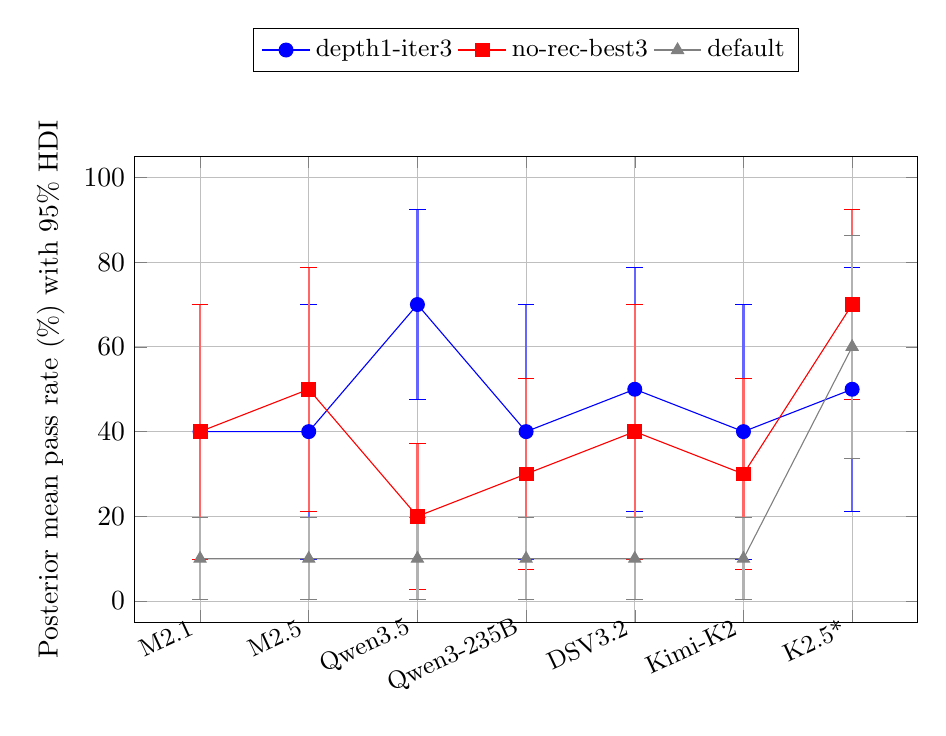
\begin{tikzpicture}
\begin{axis}[
  width=0.95\linewidth,
  height=7.5cm,
  ymin=-5, ymax=105,
  ylabel={Posterior mean pass rate (\%) with 95\% HDI},
  symbolic x coords={M2.1,M2.5,Qwen3.5,Qwen3-235B,DSV3.2,Kimi-K2,K2.5*},
  xtick=data,
  x tick label style={rotate=25,anchor=east,font=\small},
  legend style={at={(0.5,1.18)},anchor=south,legend columns=4,font=\small},
  grid=major,
]
% depth1-iter3 (dominant mode for most)
\addplot[blue,mark=*,mark size=2.5pt,
  error bars/.cd,y dir=both,y explicit,
  error bar style={blue!60,thick},
  error mark options={rotate=90,mark size=3pt,blue}]
  coordinates {
    (M2.1,40) +- (0,30.1)
    (M2.5,40) +- (0,30.1)
    (Qwen3.5,70) +- (0,22.5)
    (Qwen3-235B,40) +- (0,30.1)
    (DSV3.2,50) +- (0,28.8)
    (Kimi-K2,40) +- (0,30.1)
    (K2.5*,50) +- (0,28.8)
  };
% no-rec-best3
\addplot[red,mark=square*,mark size=2.5pt,
  error bars/.cd,y dir=both,y explicit,
  error bar style={red!60,thick},
  error mark options={rotate=90,mark size=3pt,red}]
  coordinates {
    (M2.1,40) +- (0,30.1)
    (M2.5,50) +- (0,28.8)
    (Qwen3.5,20) +- (0,17.2)
    (Qwen3-235B,30) +- (0,22.5)
    (DSV3.2,40) +- (0,30.1)
    (Kimi-K2,30) +- (0,22.5)
    (K2.5*,70) +- (0,22.5)
  };
% default (d0-i1)
\addplot[gray,mark=triangle*,mark size=2.5pt,
  error bars/.cd,y dir=both,y explicit,
  error bar style={gray!60,thick},
  error mark options={rotate=90,mark size=3pt,gray}]
  coordinates {
    (M2.1,10) +- (0,9.7)
    (M2.5,10) +- (0,9.7)
    (Qwen3.5,10) +- (0,9.7)
    (Qwen3-235B,10) +- (0,9.7)
    (DSV3.2,10) +- (0,9.7)
    (Kimi-K2,10) +- (0,9.7)
    (K2.5*,60) +- (0,26.3)
  };
\legend{depth1-iter3,no-rec-best3,default}
\end{axis}
\end{tikzpicture}
\caption{Bayesian 95\% HDI for pass rate by model and mode. Points show posterior mean; bars show 95\% credible interval under Beta(1,1) prior. For pre-fix models, default (gray) clusters at 10\% while scaffolded modes separate. K2.5 (post-fix) shows overlapping intervals across all modes.}
\label{fig:bayesian-hdi}
\end{figure}

\subsection{Thompson Sampling Mode Selection}

To formalize mode selection under uncertainty, we apply Thompson sampling---a Bayesian multi-armed bandit algorithm. Each mode is an arm with Beta posterior parameters from observed data. Over 10{,}000 simulated rounds per model, we record the fraction of rounds each mode is selected as optimal.

\begin{table}[t]
\centering
\caption{Thompson sampling selection probability per model (10{,}000 rounds). Bold indicates the mode most frequently selected as optimal.}
\label{tab:thompson-sampling}
\begin{tabular}{lrrrr}
\toprule
Model & default & depth1-iter3 & depth6-single & no-rec-best3 \\
\midrule
M2.1 & 0.010 & \textbf{0.490} & 0.009 & 0.491 \\
M2.5 & 0.005 & 0.318 & 0.004 & \textbf{0.672} \\
Qwen3.5 & 0.001 & \textbf{0.991} & 0.001 & 0.008 \\
Qwen3-235B & 0.020 & \textbf{0.666} & 0.016 & 0.298 \\
DSV3.2 & 0.005 & \textbf{0.676} & 0.005 & 0.314 \\
Kimi-K2 & 0.020 & \textbf{0.666} & 0.016 & 0.298 \\
\midrule
\multicolumn{5}{l}{\emph{Post-FINAL-fix:}} \\
K2.5* & 0.205 & 0.069 & 0.207 & \textbf{0.519} \\
\midrule
Macro-avg & 0.038 & \textbf{0.554} & 0.037 & 0.372 \\
\bottomrule
\end{tabular}
\end{table}

\begin{figure}[t]
\centering
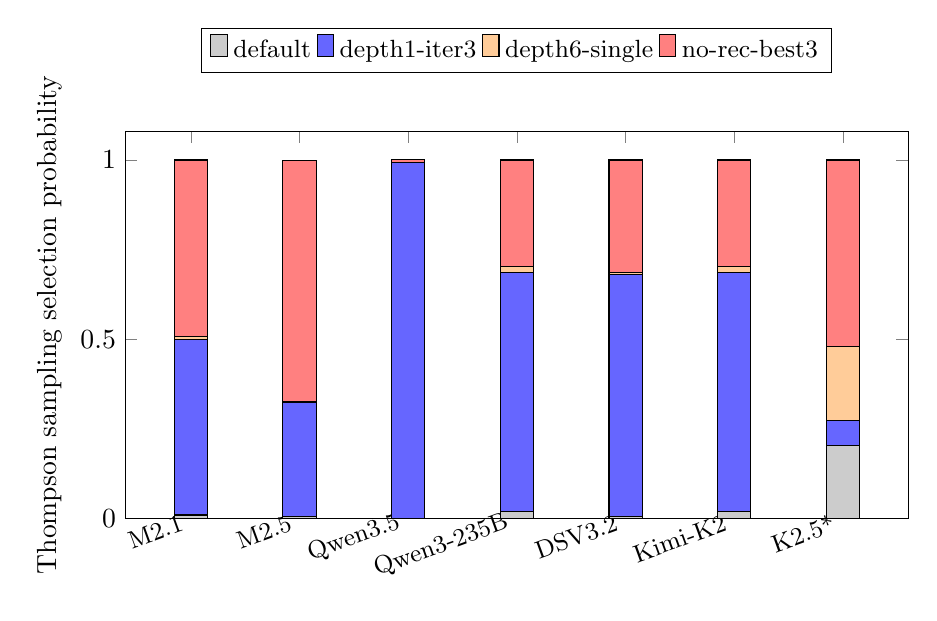
\begin{tikzpicture}
\begin{axis}[
  ybar stacked,
  bar width=12pt,
  width=0.95\linewidth,
  height=6.5cm,
  ymin=0, ymax=1.08,
  ylabel={Thompson sampling selection probability},
  symbolic x coords={M2.1,M2.5,Qwen3.5,Qwen3-235B,DSV3.2,Kimi-K2,K2.5*},
  xtick=data,
  x tick label style={rotate=20,anchor=east,font=\small},
  legend style={at={(0.5,1.15)},anchor=south,legend columns=4,font=\small},
]
\addplot[fill=gray!40] coordinates {(M2.1,0.010) (M2.5,0.005) (Qwen3.5,0.001) (Qwen3-235B,0.020) (DSV3.2,0.005) (Kimi-K2,0.020) (K2.5*,0.205)};
\addplot[fill=blue!60] coordinates {(M2.1,0.490) (M2.5,0.318) (Qwen3.5,0.991) (Qwen3-235B,0.666) (DSV3.2,0.676) (Kimi-K2,0.666) (K2.5*,0.069)};
\addplot[fill=orange!40] coordinates {(M2.1,0.009) (M2.5,0.004) (Qwen3.5,0.001) (Qwen3-235B,0.016) (DSV3.2,0.005) (Kimi-K2,0.016) (K2.5*,0.207)};
\addplot[fill=red!50] coordinates {(M2.1,0.491) (M2.5,0.672) (Qwen3.5,0.008) (Qwen3-235B,0.298) (DSV3.2,0.314) (Kimi-K2,0.298) (K2.5*,0.519)};
\legend{default,depth1-iter3,depth6-single,no-rec-best3}
\end{axis}
\end{tikzpicture}
\caption{Thompson sampling mode allocation per model. Concentrated bars indicate high confidence in a single mode; diffuse bars indicate mode-insensitivity. Qwen3.5 is $>99\%$ concentrated on depth1-iter3; K2.5 (post-fix) is nearly uniformly distributed. Across pre-fix models, attempt-rich modes (blue + red) capture $>96\%$ of selections.}
\label{fig:thompson-allocation}
\end{figure}

Three patterns emerge from the Thompson analysis. First, \textbf{depth1-iter3 is the aggregate optimal mode} (55.4\% selection across models), confirming shallow recursion with attempts as the best general recommendation. Second, \textbf{model--mode interaction is extreme}: Qwen3.5 selects depth1-iter3 in 99.1\% of rounds, while M2.5 selects no-rec-best3 in 67.2\%---the ``best mode'' genuinely depends on the model. Third, \textbf{deep single-pass and unscaffolded modes are never selected} ($<2\%$ for pre-fix models), formalizing the finding that attempt budget is a prerequisite for competitive performance.

\subsection{Latency Variability}

Response time stability matters for deployment SLAs. We measure the coefficient of variation (CV = std/mean) across the 8 tasks per configuration.

\begin{table}[t]
\centering
\caption{Latency variability for selected configurations (seconds). Low CV indicates stable response times.}
\label{tab:latency-cv}
\begin{tabular}{llrrrrr}
\toprule
Model & Mode & Mean & Std & CV & Min & Max \\
\midrule
Qwen3.5 & depth1-iter3 & 11.9 & 5.2 & 0.44 & 5.5 & 23.4 \\
Qwen3.5 & default & 11.4 & 6.5 & 0.57 & 4.3 & 23.5 \\
M2.1 & depth1-iter3 & 7.4 & 3.6 & 0.48 & 3.1 & 14.4 \\
DSV3.2 & default & 31.5 & 10.4 & 0.33 & 12.3 & 50.4 \\
Kimi-K2 & depth6-single & 23.0 & 22.7 & 0.98 & 7.1 & 72.5 \\
K2.5* & depth1-iter3 & 28.6 & 23.3 & 0.81 & 8.4 & 86.2 \\
\bottomrule
\end{tabular}
\end{table}

\begin{figure}[t]
\centering
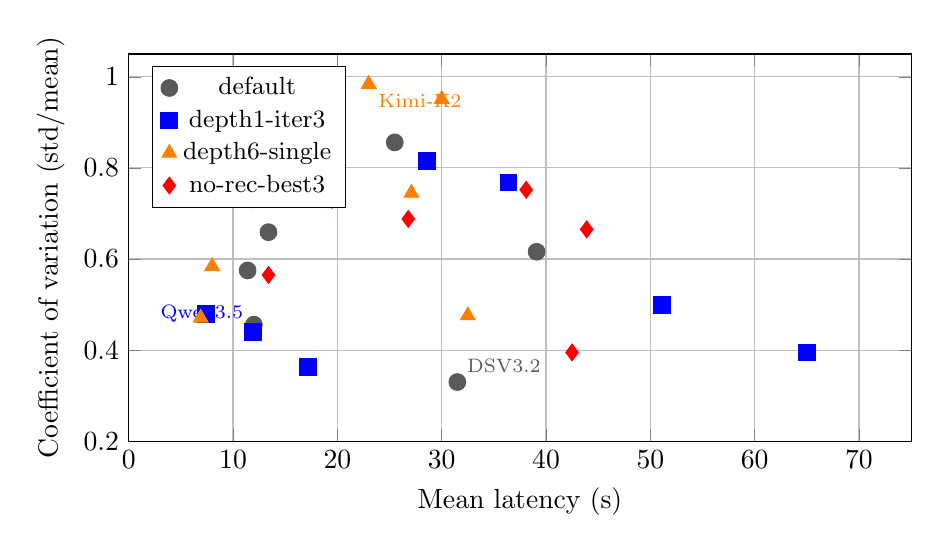
\begin{tikzpicture}
\begin{axis}[
  width=0.95\linewidth,
  height=6.5cm,
  xlabel={Mean latency (s)},
  ylabel={Coefficient of variation (std/mean)},
  xmin=0, xmax=75,
  ymin=0.2, ymax=1.05,
  grid=major,
  legend style={at={(0.03,0.97)},anchor=north west,font=\small},
]
% default (d0-i1)
\addplot[only marks,mark=*,mark size=3pt,gray!70!black] coordinates {
  (11.9,0.731) (13.4,0.659) (25.5,0.856) (11.4,0.575) (31.5,0.330) (12.0,0.456) (39.1,0.616)};
% depth1-iter3
\addplot[only marks,mark=square*,mark size=3pt,blue] coordinates {
  (7.4,0.479) (17.2,0.363) (36.4,0.768) (11.9,0.440) (51.1,0.499) (65.0,0.395) (28.6,0.815)};
% depth6-single
\addplot[only marks,mark=triangle*,mark size=3pt,orange] coordinates {
  (6.9,0.471) (8.0,0.584) (30.0,0.951) (12.9,0.791) (32.5,0.476) (23.0,0.984) (27.1,0.745)};
% no-rec-best3
\addplot[only marks,mark=diamond*,mark size=3pt,red] coordinates {
  (12.0,0.782) (13.4,0.565) (43.9,0.665) (19.5,0.730) (42.5,0.395) (26.8,0.688) (38.1,0.752)};
\legend{default,depth1-iter3,depth6-single,no-rec-best3}
% Annotate Pareto-optimal point
\node[anchor=south east,font=\scriptsize,blue] at (axis cs:11.9,0.440) {Qwen3.5};
\node[anchor=south west,font=\scriptsize,gray!70!black] at (axis cs:31.5,0.330) {DSV3.2};
\node[anchor=north west,font=\scriptsize,orange] at (axis cs:23.0,0.984) {Kimi-K2};
\end{axis}
\end{tikzpicture}
\caption{Latency mean vs coefficient of variation by model and mode. Ideal configurations are in the lower-left quadrant. Qwen3.5 with depth1-iter3 (blue, 11.9s, CV=0.44) combines low latency with moderate stability. Deep single-pass modes (orange) tend toward high CV.}
\label{fig:latency-cv}
\end{figure}

CV ranges from 0.33 (DSV3.2 default, most stable) to 0.98 (Kimi-K2 depth6-single, most variable). Two observations are deployment-relevant. First, \textbf{deeper modes tend toward higher CV}: depth6-single-pass has mean CV=0.72 across models vs 0.60 for depth1-iter3, suggesting that deep recursion introduces timing unpredictability from variable sub-call chains. Second, \textbf{Qwen3.5 with depth1-iter3 is Pareto-optimal for latency stability}: it achieves the best combination of low mean (11.9s), moderate CV (0.44), and high pass rate (75\%), making it the strongest candidate for latency-sensitive deployment.

\section{Implementation Architecture}

Axon's architecture extends the core RLM recursive-decomposition pattern \cite{zhang2025rlm} with explicit state-management operators for checkpointed exploratory search. The key architectural difference from standard RLM is the addition of fork/checkpoint/VFS primitives that enable branch-local reasoning state.

\begin{figure}[t]
\centering
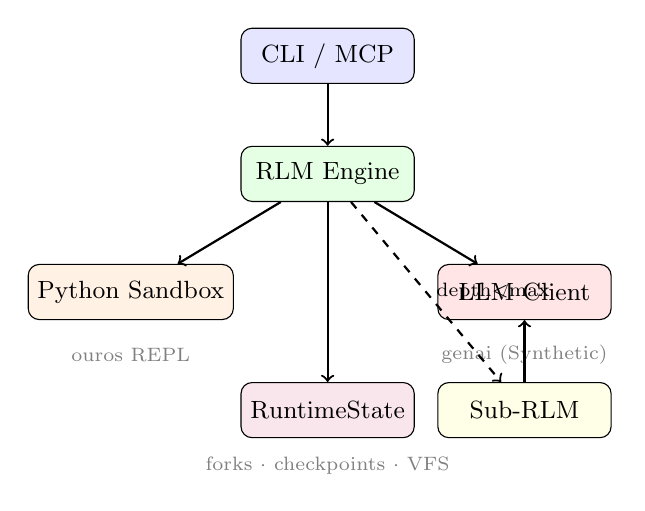
\begin{tikzpicture}[
  block/.style={draw,rounded corners,minimum width=2.2cm,minimum height=0.7cm,font=\small},
  every node/.style={font=\small}
]
\node[block,fill=blue!10] (cli) at (0,5) {CLI / MCP};
\node[block,fill=green!10] (rlm) at (0,3.5) {RLM Engine};
\node[block,fill=orange!10] (sandbox) at (-2.5,2) {Python Sandbox};
\node[block,fill=red!10] (llm) at (2.5,2) {LLM Client};
\node[block,fill=purple!10] (state) at (0,0.5) {RuntimeState};
\node[block,fill=yellow!10] (sub) at (2.5,0.5) {Sub-RLM};

\node[font=\scriptsize,text=gray] at (-2.5,1.2) {ouros REPL};
\node[font=\scriptsize,text=gray] at (2.5,1.2) {genai (Synthetic)};
\node[font=\scriptsize,text=gray] at (0,-0.2) {forks $\cdot$ checkpoints $\cdot$ VFS};

\draw[->,thick] (cli) -- (rlm);
\draw[->,thick] (rlm) -- (sandbox);
\draw[->,thick] (rlm) -- (llm);
\draw[->,thick] (rlm) -- (state);
\draw[->,thick,dashed] (rlm) -- node[right,font=\scriptsize]{depth$<$max} (sub);
\draw[->,thick] (sub) -- (llm);
\end{tikzpicture}
\caption{Axon architecture. The RLM engine orchestrates iteration loops over a Python sandbox (ouros) and LLM client (genai), with RuntimeState managing fork/checkpoint/VFS state. When depth $<$ max\_depth, \texttt{llm\_query()} spawns a child RLM with its own sandbox.}
\label{fig:architecture}
\end{figure}

The checkpoint/fork mechanism allows the model to create snapshots of its reasoning state and branch into parallel exploration paths. Each fork maintains its own VFS (virtual file system) for scratch state, enabling the model to write intermediate results without cross-contaminating other branches. When a branch fails, the model can restore to a prior checkpoint and try an alternative strategy. This design makes the recursion framework more robust to early reasoning errors compared to pure linear recursion.

\section{Answer to the Research Question}
Under current measured evidence, the strongest defensible answer is:

\begin{quote}
For short-horizon tasks, recursion is \emph{not} uniformly beneficial by itself. Gains are mostly explained by attempt budget and evaluation/runtime policy; shallow recursion with sufficient iterations can outperform baselines, but non-recursive best-of-3 is already a strong competitor.
\end{quote}

This is compatible with \rlm literature in spirit \cite{zhang2025rlm,primeintellect2026rlm}, but narrower in scope: our results are about practical profile behavior under strict checkers, not a universal claim that deeper recursion improves all task classes.

\section{Threats to Validity}
\paragraph{Internal validity.}
Observed improvements combine multiple interventions (typed checking, runtime hardening, prompt contract changes) and cannot be attributed to recursion alone without larger controlled factorial studies.
Checkpoint/fork/workspace controls are available in all modes but are not independently ablated, so causal attribution to these controls is out of scope for current results.

\paragraph{External validity.}
HF and Codeforces analyses rely on small slices (40 and 8 runs). These are useful diagnostic instruments but insufficient for strong generalization.

\paragraph{Construct validity.}
Strict executable scoring conflates algorithmic errors with formatting and compilation discipline. The compile taxonomy partially separates these factors but not perfectly.

\paragraph{Statistical conclusion validity.}
Many confidence intervals are wide due to low sample counts. Claims are therefore directional unless supported by higher-sample runs.

\section{Future Work: Plan Annealing for Recursive Coordination}
A concrete next step is plan annealing: explicit progress propagation across recursive calls so sub-LLMs receive only unresolved objectives.

\begin{lstlisting}[language={}]
PLAN = [{task, state}]  # state in {pending, in_progress, done, blocked}
for each recursive handoff:
  update PLAN using newly verified evidence
  ACTIVE = [item for item in PLAN if item.state != done]
  child_input = {active_tasks: ACTIVE, constraints, failure_notes, key evidence}
  child_output = sub_llm(child_input)
  merge child_output states back into PLAN
\end{lstlisting}

This mechanism is aligned with emerging evidence that stable internal structure, not only depth, matters for long reasoning quality \cite{chen2026molecular}. Evaluation should test whether plan annealing lowers token use per solved task, reduces timeout/error rate, and improves strict executable pass rate at fixed budgets.

\section{Conclusion}
This paper reframes \axon evaluation around a practical question from \rlm deployment: recursion versus extra iterations on short-horizon tasks. A multi-model Pareto analysis across seven Synthetic-hosted models (224 runs) yields three main conclusions.

First, \textbf{scaffold bugs can masquerade as model limitations}. A FINAL-extraction bug in the fallback path caused depth6-single-pass to score 0\% across all pre-fix models, even when the underlying answers were correct. After fixing, Kimi-K2.5 achieved 62.5\% in depth6-single-pass---demonstrating that deep recursion can work when the scaffold faithfully surfaces model outputs.

Second, \textbf{the Pareto frontier has two co-dominant configurations}: Qwen3.5-397B with depth1-iter3 (75\% pass, 11.9s, \$0.0044/task---best speed and cost) and Kimi-K2.5 with no-rec-best3 (75\% pass, 38.1s, \$0.0064/task---best single-pass robustness at 62.5\% even in default mode). Speed varies 10$\times$ across models (7.4s to 71.7s), making latency a first-order deployment concern.

Third, \textbf{whether recursion or iteration wins is model-dependent}: Qwen3.5 strongly favors recursion (75\% vs 12.5\%) while MiniMax-M2.5 favors iteration (50\% vs 37.5\%), and Kimi-K2.5 is relatively mode-insensitive (50--75\% across all modes). This interaction effect between model capability and scaffold mode is a new finding that cautions against universal mode recommendations.

\bibliographystyle{plain}
\bibliography{refs}

\end{document}
